\RequirePackage[OT1]{fontenc}
\documentclass[conference]{IEEEtran}
\usepackage{amsmath,amssymb,graphicx,booktabs,array,tabularx,xurl,placeins,cite}
\usepackage[hidelinks]{hyperref}
\title{MarsPro: Missing-Label-Aware Multi-Stress-Associated Protein Prediction and Domain-Adapted Inverse Folding}
\author{}
\begin{document}
\maketitle



\begin{abstract}
Pooling stress-specific protein resources creates missing labels: a sequence observed for one condition is usually unknown, not negative, for the others. \textbf{MarsPro} combines MarsDataset, a provenance-aware 40,000-sequence resource; MarsClass, a six-output sequence predictor; and MarsMPNN, a domain-adapted inverse-folding model. Sequence--task cells record positive, source-comparator zero, or unknown evidence; task-normalized Masked-BCE and shared LoRA exclude unknown cells from supervision. MarsClass reaches 0.9771 validation macro AP versus 0.9539 for unknown-as-negative encoding and 0.9753 on a locked test. Four complete-source folds remain above prevalence (AP 0.198--0.903; baselines 0.108--0.437). Across 798 backbones and three matched seeds, MarsMPNN reduces reference STNQDE and Met/Cys surface distances by 16.67\% and 17.30\% with similar pLDDT and US-align RMSD. On 1,000 distinct fixed-test ID50 clusters, frozen MarsClass rescoring rises from 0.6185 to 0.6725, with 731/1,000 backbones improving. The resulting workflow supports traceable experimental candidate prioritization.
\end{abstract}

\begin{IEEEkeywords}protein language models; incomplete labels; multi-label learning; low-rank adaptation; ProteinMPNN; inverse folding; extremophile proteins.\end{IEEEkeywords}

\section{Introduction}\label{sec:intro}

Terrestrial extremophiles inform astrobiology and supply sequence diversity for biotechnology under low temperature, salinity, desiccation, oxidative chemistry, and radiation-associated stress \cite{ref14,ref15,ref31,ref32}. Computational discovery has progressed from composition features to protein language models (PLMs), including ESM, ProtTrans, and Ankh \cite{ref16,ref2,ref17}. This progress increases representation capacity, but it does not resolve a central data problem: a protein collected for one stress category is usually unobserved, rather than negative, for the others.

Most predictors remain task specific. HaloClass and HPClas target halophilic proteins \cite{ref1,ref18}; ESM-PsyPred and related models address psychrophilic proteins or enzymes \cite{ref20,ref21}; AHAPC combines three extremophile classes \cite{ref19}; other systems predict antioxidant or DNA-repair proteins \cite{ref22,ref23,ref24}. Their label spaces and comparator definitions cannot be directly merged into a fully observed table.

The obstacle is therefore not simply model capacity. Pooling task-specific resources produces a sparse sequence--task matrix whose zeros and unknowns have different meanings. A joint predictor must preserve that distinction while allowing shared and task-specific representations to be compared on the same observed cells. Sequence design introduces a complementary objective: generated sequences must be assessed for structural preservation and movement toward the intended surface composition. The data model, loss, generator, and assessment endpoints therefore form one evidence-preserving workflow.

MarsPro preserves this evidence model from resource construction through design assessment (Fig.~\ref{fig:1}). Its contributions are MarsDataset, a traceable 40,000-sequence, six-task resource; MarsClass, a shared-LoRA six-output predictor evaluated across three PLMs, mask controls, locked tests, and complete-source folds; and MarsMPNN, an inverse-folding model assessed with 4,788 matched-seed refolds plus frozen MarsClass rescoring on 1,000 fixed-test ID50 clusters. Labels denote source, family, or proteome membership rather than measured tolerance.

\begin{figure*}[!t]
\centering
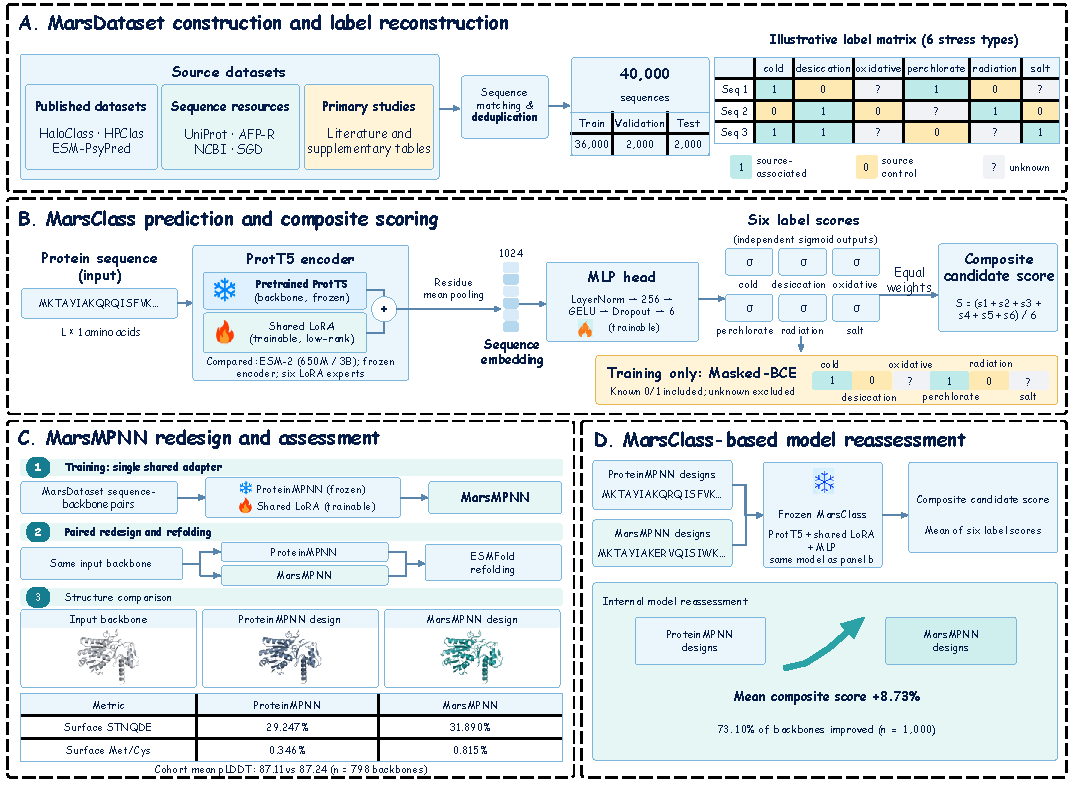
\includegraphics[width=\textwidth]{figures/framework.pdf}
\caption{MarsPro prediction--design--rescoring framework. MarsDataset supports MarsClass six-label prediction and MarsMPNN backbone-conditioned adaptation. The structural branch uses 7,979 candidates, 798 held-out backbones, and three matched design seeds; a separate frozen-MarsClass challenge uses 1,000 distinct fixed-test ID50 clusters.}
\label{fig:1}
\end{figure*}

\section{Related Work}\label{sec:related}

\subsection{Extreme-Environment Resources and Predictors}
Extremophile resources range from measured enzymes to family members and proteins drawn from adapted organisms, so their entries carry different evidence strengths. Mars-analog studies provide environmental context \cite{ref14,ref15}, whereas CAPP illustrates large-scale cold-adapted sequence collection \cite{ref31}. Task predictors span HPClas, HaloClass, AHAPC, ESM-PsyPred, and models for psychrophilic enzymes, antioxidant proteins, and DNA repair \cite{ref1,ref18,ref20,ref21,ref19,ref22,ref23,ref24}. MarsDataset preserves provenance for curation and stratified evaluation, while MarsClass predicts source-associated membership from sequence alone.

\subsection{PLMs and Parameter-Efficient Adaptation}
ESM, ProtTrans, and Ankh learn transferable sequence representations \cite{ref16,ref2,ref17}, and ESMFold links PLMs to structure prediction \cite{ref3}. LoRA learns compact low-rank updates while freezing pretrained weights \cite{ref4}. We use it to compare one shared six-output adapter with six task-specific adapters, without assuming that expert fusion is beneficial.

\subsection{Unknown and Partial Labels}
Positive--unlabeled and partial-label learning distinguish unobserved entries from negatives and restrict supervision to supported labels \cite{ref25,ref7}; stochastic masking has also been used for imbalance \cite{ref26}. Our narrower setting assigns each sequence--task cell as positive, source-comparator zero, or unknown. Zero-filling, random equal-count masks, row-shuffled masks, and artificial removal of known labels test whether sequence--label correspondence, rather than label count alone, explains performance.

\subsection{Structure-Conditioned Design and Assessment}
ProteinMPNN learns backbone-conditioned sequences \cite{ref5}, and HaloMPNN adapts inverse folding to halophilic proteomes \cite{ref6}. Rosetta offers complementary refinement \cite{ref27}, while FreeSASA, residue accessibility maxima, and US-align support surface and structural assessment \cite{ref9,ref10,ref11}. Pfam, HMMER, and MMseqs2 support family and relationship auditing \cite{ref28,ref29,ref30}. We separate generation, predicted structure, surface features, and frozen-predictor scores because no single layer establishes function.

\section{Dataset and Labels}

MarsDataset integrates three acquisition routes. Stable identifiers and annotation records come from UniProt, NCBI, SGD, and specialized resources. Published classification datasets and supplementary files contribute task-specific positive and comparator collections. Primary studies link proteins, families, or proteomes to their experimental or source criteria. Exact-sequence deduplication prevents repeated database hits or measurements from becoming independent proteins. Source links, taxonomy, relationship components, ID50 clusters, and Pfam/HMMER/MMseqs2 side tables preserve provenance and support audit.

The six tasks are cold, desiccation, oxidative, perchlorate, radiation, and salt. A cell is positive when the source rule supports membership, zero only when a source-supported comparator exists, and unknown otherwise. The final MarsDataset label table retains native classifier zeros and adds reviewed comparator zeros only at previously unknown cells; conflicts preserve positives. This adds 2,967 zero cells across 2,445 unique sequences and records 883 positive-priority conflicts. It does not introduce sampled pseudo-zeros. Positives, native zeros, and reviewed source zeros receive unit weight; unknowns receive zero loss weight.

\begin{table}[t]
\centering
\caption{Dataset coverage: 40,000 sequences; fixed 36,000/2,000/2,000 split.}
\label{tab:1}
\footnotesize
\setlength{\tabcolsep}{3pt}
\begin{tabularx}{\columnwidth}{@{}Xrrrrr@{}}
\toprule
Task & 1 & 0 & Unknown & Val. 1/0 & Test 1/0 \\
\midrule
cold & 4,510 & 2,661 & 32,829 & 228/131 & 229/130 \\
desiccation & 7,250 & 1,112 & 31,638 & 366/66 & 360/50 \\
oxidative & 7,175 & 2,458 & 30,367 & 356/129 & 356/124 \\
perchlorate & 2,229 & 262 & 37,509 & 111/14 & 111/11 \\
radiation & 4,583 & 6,812 & 28,605 & 226/339 & 207/364 \\
salt & 8,181 & 3,151 & 28,668 & 406/153 & 412/155 \\
\bottomrule
\end{tabularx}
\end{table}

The 40,000 sequences define 240,000 cells: 33,928 positive, 16,456 source-comparator zero, and 189,616 unknown (79.01\%). Before partitioning, the source pool was globally clustered at 50\% sequence identity and 80\% bidirectional coverage; one label-independent representative was retained per connected component. The fixed 36,000/2,000/2,000 train/validation/test splits share no registered ID50 clusters. Model and ablation comparisons use validation; the test split is evaluated once after the checkpoint and thresholds are frozen. The structural subset contains 7,979 classification-training sequences with at least one positive label and predicted structures, split into 6,383/798/798 backbones. Identifier, exact-sequence, and existing ID50 checks found no overlap from the structural test subset to structural train/validation.

\section{Methods}\label{sec:method}

\subsection{Problem Formulation}
Let $\mathcal{D}=\{(x_i,\mathbf{y}_i,\mathbf{m}_i)\}_{i=1}^N$ denote the sequence resource. Here $x_i$ is an amino-acid sequence, $\mathbf{y}_i\in\{0,1\}^T$ contains encoded observed labels, and $\mathbf{m}_i\in\{0,1\}^T$ records which of the $T=6$ tasks are observed. Entries with $m_{it}=0$ are unknown rather than negative. The predictor estimates $\mathbf{p}_i\in[0,1]^T$. The design branch conditions sequence $S$ on backbone $X$ and compares base and adapted models on registered backbone pairs.

\subsection{MarsClass: Six-Output Prediction and Masked Loss}
MarsClass takes only the amino-acid sequence as input. Source identifiers, taxonomy, Pfam assignments, and other provenance fields are excluded from model inputs and retained only for curation and stratified evaluation. For sequence $x_i$, a PLM produces residue representations; valid-residue mean pooling yields $h_i$. Layer normalization, a 256-dimensional hidden layer, GELU, dropout, and six sigmoid outputs estimate independent source-label probabilities. LoRA represents selected weights as $W=W_0+(\alpha/r)BA$, freezing $W_0$ while training low-rank factors and the classifier. Shared adaptation uses one adapter; task experts use six adapters with direct, fixed-fusion, or dynamic-fusion outputs.

Let $y_{it}\in\{0,1,?\}$ and $m_{it}=\mathbb{1}[y_{it}\ne ?]$. With binary cross-entropy $\ell_{it}$, observed count $n_t=\sum_i m_{it}$, and active tasks $\mathcal{T}_B=\{t:n_t>0\}$,
\begin{equation}\mathcal{L}_{\mathrm{mask}}=\frac{1}{|\mathcal{T}_B|}\sum_{t\in\mathcal{T}_B}\frac{\sum_i m_{it}\ell_{it}}{n_t}.\end{equation}
Task denominators are aggregated across devices. Unknown cells contribute no loss; the BCE comparator encodes them as zero. Every model comparison uses the same observed validation positions; the validation-selected model is subsequently evaluated on observed test positions without further fitting.

\subsection{MarsMPNN: Domain-Adapted ProteinMPNN}
The design branch adapts ProteinMPNN v\_48\_020 for $p_\theta(S\mid X)$ using pooled six-source data. Joint LoRA uses rank 8, scaling 16, dropout 0.05, and W1/W2/W3 plus W\_out targets. Base and adapted models each generate three sequences for 798 fixed structural-test backbones at temperature 0.1. Seeds 42, 43, and 44 are matched within every backbone and method, yielding 2,394 designs per method. The six-adapter design branch is kept outside the present joint-LoRA structural comparison.

\subsection{Refolding and Surface Features}
All 4,788 designs are refolded under identical settings \cite{ref8}. FreeSASA uses Lee--Richards calculation, ProtOr radii, a 1.4-angstrom probe, and 20 slices \cite{ref9}; relative solvent accessibility uses residue maxima \cite{ref10}. Surface residues satisfy RSA $\geq0.25$. For feature $k\in\{\mathrm{STNQDE},\mathrm{MC}\}$, reference proximity is the absolute fraction difference
\begin{equation}d_{ik}=\left|f^{\mathrm{design}}_{ik}-f^{\mathrm{ref}}_{ik}\right|.\end{equation}
Sequence recovery and novelty excluding the parent measure design conservation and departure. Mean pLDDT and pTM provide refolding-confidence diagnostics. US-align compares every design with its input backbone and reports aligned RMSD, reference-normalized TM-score, and GDT-TS \cite{ref11}.

\subsection{Fixed-Test Redesign and Frozen Rescoring}
From the fixed 2,000-sequence classification test split, 1,000 source-positive references were selected before prediction by ascending SHA256 rank, subject to canonical residues, length at most 500, and distinct registered ID50 clusters. No selected reference has an exact-sequence, registered ID50-cluster, or registered relationship-component overlap with classification train/validation; references also exclude exact and registered ID50 overlap with the 10,000-structure ProteinMPNN corpus. ESMFold generated all 1,000 input backbones. ProteinMPNN and MarsMPNN then produced matched designs at seeds 42, 43, and 44 on each backbone.

The frozen epoch-5 MarsClass checkpoint scores the 1,000 references and 6,000 designs without retraining or result-dependent selection. Its aggregate is $S(x)=\frac{1}{6}\sum_{t=1}^6p_t(x)$, and $\Delta S_i=S(x_i^{\mathrm{Mars}})-S(x_i^{\mathrm{base}})$. Seed-level scores are first averaged within each backbone, making the 1,000 backbones the analysis units. We report paired aggregate change, change over the reference-positive labels, improvement fraction, and six-dimensional prediction distance to the corresponding reference.

\section{Experimental Protocol}\label{sec:experiments}

Evaluation follows the two dependencies in the framework. The prediction study first tests whether evidence-aware masking improves observed-label performance and whether a shared adapter retains the accuracy of six task experts. The design study then measures how domain adaptation changes registered surface and structural endpoints before asking whether the frozen predictor gives a consistent post-hoc ranking signal.

Classification covers 21 primary configurations and two controls: ProtT5 and ESM-2 (650M/3B), frozen or LoRA encoders, BCE or Masked-BCE, ProtT5 experts/fusion, six AAC logistic regressions, and LightGBM/random forests on 582 handcrafted features \cite{ref12,ref13}. Rich features combine length and log length, AAC, dipeptide composition, k-spaced amino-acid group pairs, and physicochemical groups. Deep checkpoints are selected by validation macro AP over five epochs, and validation also determines F1/MCC thresholds. Mask controls use rank 8, scaling 16, dropout 0.05, query/value adaptation, FP16, effective batch 16, and matched seeds 42--44. Frozen ProtT5 uses five epochs, seed 42, and effective batch 64; the three-seed mask experiment remains separate from the primary comparison. After selecting shared ProtT5-LoRA with Masked-BCE, its epoch-5 checkpoint and six validation thresholds were frozen. The locked-test inference file contained only sequence identifiers and sequences; the six-output probability file was hash-sealed before test labels were joined, and no model or threshold was changed afterward.

Four predeclared source folds remove AAC or ESM-PsyPred cold, AOP2020 oxidative, or HaloClass salt plus registered ID50 clusters/components from train/validation, retrain five epochs at seed 42, and evaluate known cells once. Unknowns remain masked; prevalence is random AP.

The 2,000 validation sequences contain 2,525 observed and 9,475 unknown cells; the 2,000 test sequences contain 2,509 observed (1,675 positive and 834 zero) and 9,491 unknown cells. Only observed cells enter AP, AUROC, F1, MCC, recall, and 10-bin ECE. Random equal-count masks preserve per-task counts, row-shuffled masks preserve row/column totals, and artificial missingness removes 25\% of known training labels.

Structural analyses contain 2,394 same-backbone, same-seed pairs. Metrics are first averaged over seeds 42--44 within each backbone, leaving 798 independent analysis units. We report paired means, improvement fractions, 10,000 backbone bootstrap intervals, and Wilcoxon tests with Benjamini--Hochberg correction. All 4,788 structures complete the primary endpoints without missing values. The fixed-test rescoring challenge uses 1,000 backbone-level averages over three matched seeds, 10,000 paired bootstrap replicates, and a two-sided sign test; task-specific estimates are restricted to references positive for that task.

\section{Results}\label{sec:results}

\subsection{Unknown-Aware Learning Improves Prediction}
\begin{table*}[t]
\centering
\caption{Controlled encoder, adaptation, and supervision comparison on observed validation labels. The best value in each metric is bold.}
\label{tab:2}
\footnotesize
\setlength{\tabcolsep}{3pt}
\begin{tabularx}{\textwidth}{@{}Xllrrrr@{}}
\toprule
Backbone / features & Adaptation & Supervision & AP & AUROC & F1 & MCC \\
\midrule
\textbf{ProtT5} & \textbf{LoRA} & \textbf{Masked-BCE} & \textbf{0.9771} & \textbf{0.9623} & \textbf{0.9328} & \textbf{0.7934} \\
ProtT5 & LoRA & BCE & 0.9539 & 0.9083 & 0.8674 & 0.6204 \\
ProtT5 & Frozen & Masked-BCE & 0.9741 & 0.9570 & 0.9275 & 0.7882 \\
ProtT5 & Frozen & BCE & 0.9507 & 0.8979 & 0.8652 & 0.6084 \\
\midrule
ESM-2 3B & LoRA & Masked-BCE & 0.9749 & 0.9570 & 0.9298 & 0.7931 \\
ESM-2 3B & LoRA & BCE & 0.9509 & 0.8936 & 0.8611 & 0.5867 \\
ESM-2 3B & Frozen & Masked-BCE & 0.9734 & 0.9548 & 0.9258 & 0.7681 \\
ESM-2 3B & Frozen & BCE & 0.9468 & 0.8899 & 0.8592 & 0.5842 \\
\midrule
ESM-2 650M & LoRA & Masked-BCE & 0.9725 & 0.9550 & 0.9217 & 0.7588 \\
ESM-2 650M & LoRA & BCE & 0.9461 & 0.8868 & 0.8562 & 0.5735 \\
ESM-2 650M & Frozen & Masked-BCE & 0.9702 & 0.9507 & 0.9220 & 0.7553 \\
ESM-2 650M & Frozen & BCE & 0.9430 & 0.8803 & 0.8537 & 0.5696 \\
\midrule
Handcrafted & LightGBM & Known labels & 0.9353 & 0.8856 & 0.8757 & 0.5968 \\
Handcrafted & RF & Known labels & 0.9189 & 0.8424 & 0.8349 & 0.4959 \\
Length + AAC & LR & Known labels & 0.8970 & 0.8179 & 0.8095 & 0.4694 \\
\bottomrule
\end{tabularx}
\end{table*}

\begin{figure*}[!t]
\centering
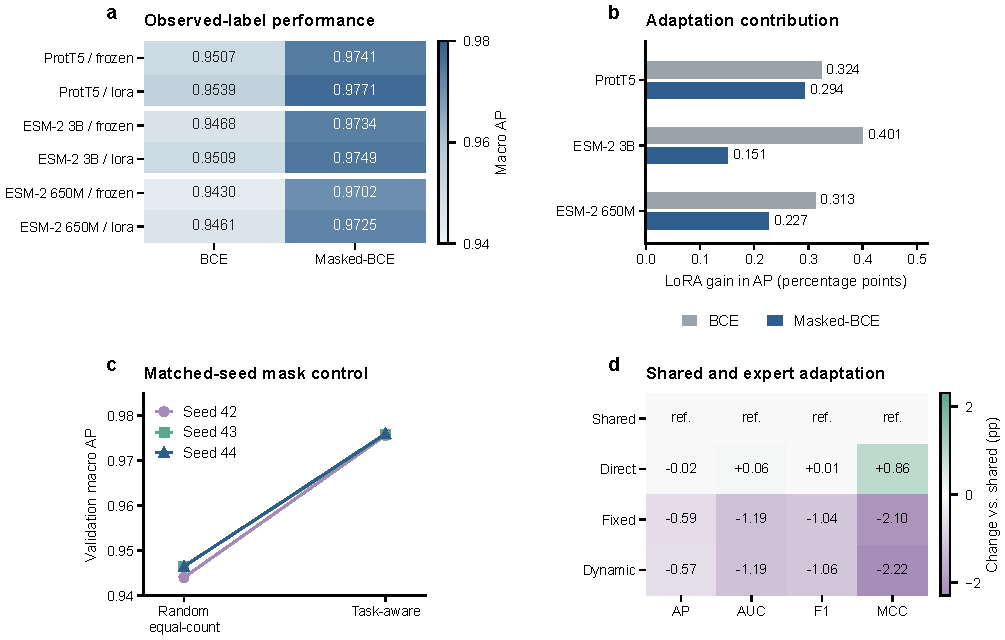
\includegraphics[width=\textwidth]{figures/ablation.pdf}
\caption{Prediction ablations on observed validation labels. (a) Macro AP across backbones, adaptations, and losses. (b) LoRA gains over frozen encoders, in percentage points. (c) Matched seeds 42--44 in the separate mask-control experiment. (d) Expert-minus-shared metric differences, in percentage points; the shared row is the reference. Panels a, b, and d report single-run comparisons.}
\label{fig:2}
\end{figure*}

Table~\ref{tab:2} is a controlled encoder-selection experiment: all neural rows use the same data split, label semantics, and evaluation positions while varying the PLM backbone, parameter adaptation, and supervision rule. Shared ProtT5-LoRA with Masked-BCE achieves the highest validation macro AP (0.9771), with AUROC 0.9623, F1 0.9328, and MCC 0.7934. LoRA adds 0.00294, 0.00227, and 0.00151 AP over frozen ProtT5, ESM-2 650M, and ESM-2 3B under masked supervision. Masked-BCE improves every frozen and LoRA backbone; for shared ProtT5-LoRA it adds 0.02315 AP and 0.17304 MCC over zero-filled BCE.

After model selection was frozen, the selected shared model obtained 0.97529 macro AP, 0.96003 macro AUROC, 0.91756 macro F1, and 0.74118 macro MCC on the one-time locked test. Micro AP was 0.98210. Macro AP changed by $-0.00180$ from validation, while the larger reductions in F1 ($-0.01522$) and MCC ($-0.05225$) indicate modest threshold-level shift despite stable ranking. Per-task test AP was 0.96958 (cold), 0.99552 (desiccation), 0.98162 (oxidative), 0.99937 (perchlorate), 0.92124 (radiation), and 0.98439 (salt). Perchlorate has only 11 observed test zeros and is interpreted with that denominator.

\subsection{Complete-Source Generalization}
The AAC-cold, ESM-PsyPred-cold, AOP2020-oxidative, and HaloClass-salt folds contain 1,392, 1,924, 1,566, and 4,095 known-label sequences. AP/prevalence is 0.327/0.175, 0.198/0.161, 0.226/0.108, and 0.903/0.437; AUROC is 0.691, 0.657, 0.736, and 0.946. All rank above random, but validation-threshold negative recall spans 0.047--0.741 and MCC 0.063--0.234, supporting cross-source ranking rather than a source-invariant threshold.

\subsection{Shared Adaptation Matches Task Experts}
\begin{table*}[t]
\centering
\caption{ProtT5 ablations on observed validation labels. Lower block reports the later mask-control batch; multi-seed cells are means, AP SD is sample standard deviation.}
\label{tab:3}
\footnotesize
\setlength{\tabcolsep}{3pt}
\begin{tabularx}{\textwidth}{@{}Xrrrrrr@{}}
\toprule
Setting & Runs & AP & AUROC & F1 & MCC & AP SD \\
\midrule
Shared LoRA & 1 & 0.97709 & 0.96227 & 0.93278 & 0.79342 & -- \\
Six experts: direct & 1 & 0.97686 & 0.96286 & 0.93285 & 0.80207 & -- \\
Six experts: fixed & 1 & 0.97116 & 0.95032 & 0.92237 & 0.77244 & -- \\
Six experts: dynamic & 1 & 0.97138 & 0.95033 & 0.92215 & 0.77125 & -- \\
Class-balanced loss & 1 & 0.97636 & 0.95927 & 0.93030 & 0.78111 & -- \\
Internal training subset & 1 & 0.97473 & 0.95867 & 0.92483 & 0.78753 & -- \\
\midrule
Task-aware mask & 3 & 0.97579 & 0.95917 & 0.92889 & 0.78423 & 0.00017 \\
Random equal-count mask & 3 & 0.94567 & 0.88668 & 0.85101 & 0.58332 & 0.00143 \\
Row-shuffled mask & 1 & 0.94088 & 0.87504 & 0.82214 & 0.54072 & -- \\
25\% known-label masking & 1 & 0.97504 & 0.95665 & 0.92808 & 0.77836 & -- \\
\bottomrule
\end{tabularx}
\end{table*}

Six direct experts reach 0.97686 macro AP, only 0.00023 below shared LoRA; fixed and dynamic fusion reach 0.97116 and 0.97138. Shared adaptation therefore provides the best AP with one adapter, although direct experts remain competitive on other metrics.

Task-aware masking averages $0.97579\pm0.00017$ macro AP across seeds, versus $0.94567\pm0.00143$ for random equal-count masking; row shuffling reaches 0.94088. Masking 25\% of known labels gives 0.97504 in one run. LightGBM exceeds length+AAC logistic regression, while task-aware PLMs add 0.04049 AP over LightGBM. Radiation has the lowest task AP (0.9275); perchlorate reaches 0.9991 but has only 14 observed validation zeros. Shared-model micro AP is 0.98175; observed-label macro and micro prevalence are 0.70511 and 0.67050, respectively, providing the denominator context needed to interpret AP and calibration.

\subsection{Matched-Seed Adaptation Shifts Surface Composition}
\begin{figure*}[!t]
\centering
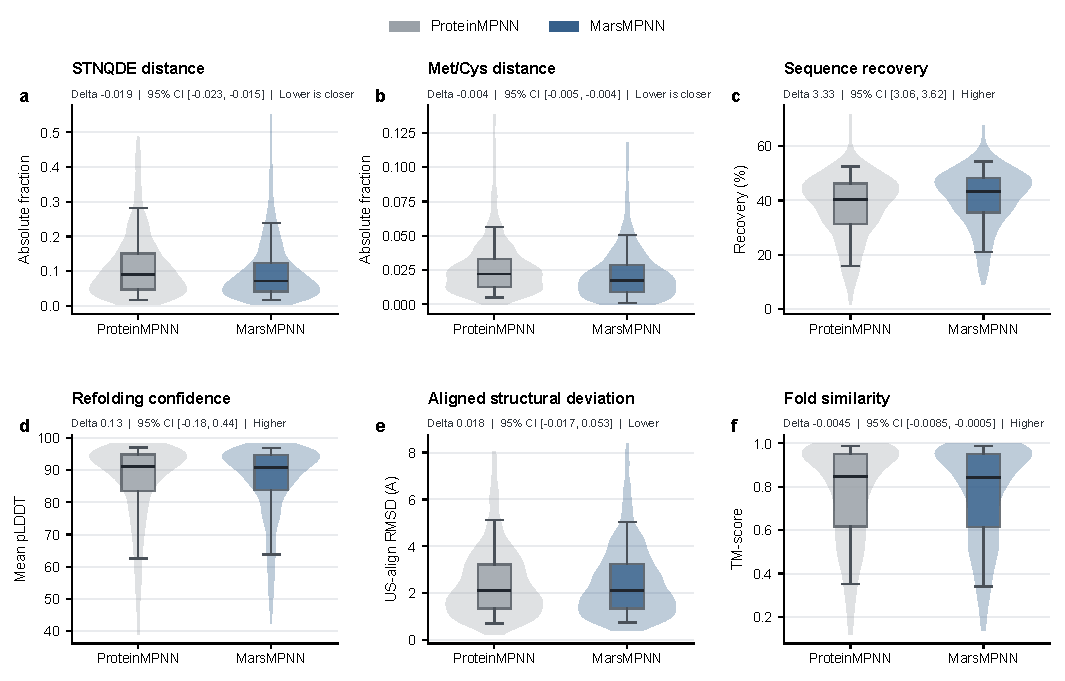
\includegraphics[width=\textwidth]{figures/design.pdf}
\caption{Matched-seed design assessment over 798 registered backbones and 2,394 paired designs. Each distribution contains one three-seed mean per backbone. (a,b) Absolute distance to the corresponding reference surface STNQDE and Met/Cys fractions. (c) Sequence recovery. (d) Mean pLDDT. (e,f) US-align RMSD and reference-normalized TM-score. Violin envelopes show density; boxes show the interquartile range and median, with whiskers spanning the 5th--95th percentiles. Insets report MarsMPNN minus ProteinMPNN mean differences and 95\% backbone-bootstrap intervals.}
\label{fig:3}
\end{figure*}

Across the matched designs, surface STNQDE rises from 29.25\% to 31.89\%. Its absolute distance to the paired reference decreases from 0.11192 to 0.09327, a 16.67\% relative reduction; 62.16\% of design pairs improve, and the backbone-level mean change is $-0.01865$ (95\% CI $[-0.02275,-0.01468]$). Surface Met/Cys rises from 0.346\% to 0.815\%, while its absolute reference distance decreases from 0.02504 to 0.02071, a 17.30\% reduction. Met/Cys distance improves in 71.89\% of pairs, with mean change $-0.00433$ (95\% CI $[-0.00468,-0.00399]$).

Sequence recovery increases from 37.91\% to 41.24\% ($+3.33$ points; 95\% CI $[3.06,3.62]$), whereas parent-excluded novelty has no clear change. Mean pLDDT is also similar (87.11 versus 87.24; difference $+0.13$, 95\% CI $[-0.18,0.44]$). US-align RMSD changes from 2.426 to 2.444~\AA{} (difference $+0.018$~\AA{}, 95\% CI $[-0.017,0.053]$). TM-score decreases slightly from 0.7700 to 0.7655 ($-0.0045$, 95\% CI $[-0.0085,-0.0005]$), and GDT-TS decreases by 0.764 points. Domain adaptation therefore shifts selected surface composition and sequence recovery while maintaining similar refolding confidence; it does not improve structural fidelity. On these training-seen references, the internal six-output mean rises from 0.6266 to 0.6687, motivating the independent fixed-test assessment below.

\subsection{Fixed-Test Rescoring Provides a Consistent Ranking Signal}
\begin{figure*}[!t]
\centering
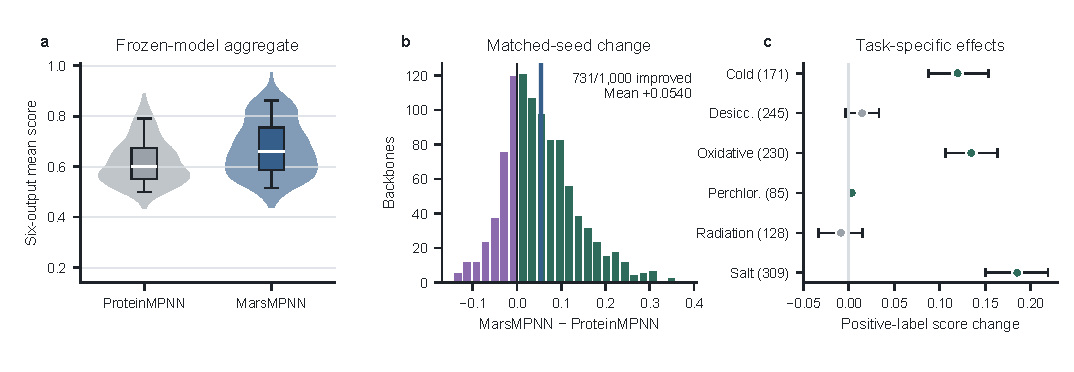
\includegraphics[width=\textwidth]{figures/rescoring.pdf}
\caption{Frozen MarsClass reassessment on 1,000 prediction-blind fixed-test references, each from a distinct registered ID50 cluster. (a) Backbone-level six-output means after averaging three matched seeds. (b) Distribution of paired MarsMPNN minus ProteinMPNN changes; the vertical line and band show the mean and 95\% paired-bootstrap interval. (c) Mean change over each reference-positive task with 95\% paired-bootstrap intervals.}
\label{fig:4}
\end{figure*}

MarsMPNN raises the backbone-averaged six-output mean from 0.61854 to 0.67251 (8.73\%); paired change is $+0.05397$ (95\% CI $[0.04889,0.05925]$, two-sided sign-test $p=6.25\times10^{-50}$). Scores improve for 731/1,000 backbones. Over only the source-positive labels of each reference, the mean rises from 0.65359 to 0.74563 ($+0.09203$; 95\% CI $[0.07757,0.10656]$), with 660/1,000 backbones improving. Six-dimensional distance to the corresponding reference prediction falls from 0.98189 to 0.83931; 700/1,000 are closer.

Task-specific positive-label changes are $+0.1196$ for cold, $+0.0145$ for desiccation, $+0.1349$ for oxidative, $+0.0033$ for perchlorate, $-0.0087$ for radiation, and $+0.1853$ for salt. Intervals exclude zero for cold, oxidative, salt, and the small near-saturated perchlorate change, but cross zero for desiccation and radiation. Thus the aggregate shift is reproducible across matched seeds but is not uniform across tasks.

\section{Discussion}\label{sec:discussion}

Masked-BCE gains across three PLMs, including frozen encoders, show that unknown-as-zero supervision is not neutral. Random and row-shuffled controls attribute the gain to correct sequence--task correspondence rather than fewer supervised cells. Six task adapters nearly match the shared model, but fusion does not improve AP. The locked test preserves within-resource ranking; complete-source retraining remains above prevalence but reveals source-dependent threshold transfer.

Relative to HaloClass \cite{ref1}, MarsPro adds explicit cross-source missingness and joint prediction; relative to HaloMPNN \cite{ref6}, it extends adaptation from one halophilic domain to pooled six-source data. Across three matched seeds, MarsMPNN reduces both selected surface-feature distances and increases sequence recovery. US-align finds unchanged RMSD and slightly lower TM-score and GDT-TS, while pLDDT remains similar. The observed effect is therefore a selective shift in sequence and surface composition, not improved structural fidelity.

The fixed-test rescoring links prediction and design on parent clusters excluded from MarsClass train/validation. Its agreement with the surface endpoint supports computational prioritization, while retaining distinct meanings: one measures a predefined compositional distance and the other measures proximity to patterns learned by the frozen MarsClass predictor. The latter is model-mediated consistency, not functional validation.

The workflow consequently returns candidates with provenance, structural diagnostics, and uncertainty rather than one opaque score. Activity, stability, solubility, and Mars-analog phenotypes remain experimental questions.

\section{Limitations}
Labels encode source, family, or proteome membership rather than measured tolerance. The four single-seed source folds cover only cold, oxidative, and salt and do not constitute taxon-, family-, or global component holdouts. Uneven comparators, composition shortcuts, and source-dependent thresholds remain relevant to deployment.

The 798 matched-seed structural-study references occur in MarsClass training. By contrast, the 1,000 rescoring references are exact-, registered-ID50-, and registered-component-disjoint from train/validation, and the 6,000 designs have no exact matches; the designs were not re-clustered against the full training set at ID50. The equal-weight aggregate is uncalibrated, perchlorate is near-saturated, and radiation and desiccation intervals cross zero.

Surface proximity is not measured activity or stability. Three matched seeds reduce sampling uncertainty, but the small decreases in TM-score and GDT-TS show that domain adaptation does not improve fold preservation. Broader source folds, ID30/family/taxon holdouts, independent evaluators, and experiments remain decisive.

\section{Conclusion}\label{sec:conclusion}
MarsPro preserves evidence status across multi-source annotation, MarsClass prediction, and MarsMPNN inverse-folding assessment. MarsClass reaches 0.9771 validation macro AP and 0.9753 on the locked test; four source folds remain above prevalence. Across 798 backbones and three matched seeds, MarsMPNN designs reduce STNQDE and Met/Cys surface-reference distances by 16.67\% and 17.30\% while maintaining similar pLDDT and US-align RMSD. On 1,000 fixed-test ID50 clusters, frozen MarsClass rescoring yields an 8.73\% higher aggregate and 73.10\% of backbone-level comparisons improve. MarsDataset, the masked objective, strict tests, and registered design analyses provide a reproducible basis for experimental candidate prioritization.

\section*{AI Assistance Disclosure}
OpenAI Codex assisted organization and numerical checks; the authors verified all evidence and conclusions.

\FloatBarrier
\begin{thebibliography}{32}
\bibitem{ref14} R. Cavicchioli, ``Extremophiles and the search for extraterrestrial life,'' \textit{Astrobiology}, vol. 2, no. 3, pp. 281--292, Aug. 2002, doi: \href{https://doi.org/10.1089/153110702762027862}{\nolinkurl{10.1089/153110702762027862}}.

\bibitem{ref15} A. G. Fair\'en \textit{et al.}, ``Astrobiology through the ages of Mars: The study of terrestrial analogues to understand the habitability of Mars,'' \textit{Astrobiology}, vol. 10, no. 8, pp. 821--843, Oct. 2010, doi: \href{https://doi.org/10.1089/ast.2009.0440}{\nolinkurl{10.1089/ast.2009.0440}}.

\bibitem{ref31} G. Varliero \textit{et al.}, ``Microbial characterisation and Cold-Adapted Predicted Protein database construction from the active layer of Greenland's permafrost,'' \textit{FEMS Microbiol. Ecol.}, vol. 97, no. 10, Art. no. fiab127, Oct. 2021, doi: \href{https://doi.org/10.1093/femsec/fiab127}{\nolinkurl{10.1093/femsec/fiab127}}.

\bibitem{ref32} K. S. Siddiqui and R. Cavicchioli, ``Cold-adapted enzymes,'' \textit{Annu. Rev. Biochem.}, vol. 75, no. 1, pp. 403--433, Jun. 2006, doi: \href{https://doi.org/10.1146/annurev.biochem.75.103004.142723}{\nolinkurl{10.1146/annurev.biochem.75.103004.142723}}.

\bibitem{ref16} A. Rives \textit{et al.}, ``Biological structure and function emerge from scaling unsupervised learning to 250 million protein sequences,'' \textit{Proc. Natl. Acad. Sci. USA}, vol. 118, no. 15, Art. no. e2016239118, Apr. 2021, doi: \href{https://doi.org/10.1073/pnas.2016239118}{\nolinkurl{10.1073/pnas.2016239118}}.

\bibitem{ref2} A. Elnaggar \textit{et al.}, ``ProtTrans: Toward understanding the language of life through self-supervised learning,'' \textit{IEEE Trans. Pattern Anal. Mach. Intell.}, vol. 44, no. 10, pp. 7112--7127, Oct. 2022, doi: \href{https://doi.org/10.1109/TPAMI.2021.3095381}{\nolinkurl{10.1109/TPAMI.2021.3095381}}.

\bibitem{ref17} A. Elnaggar \textit{et al.}, ``Ankh: Optimized protein language model unlocks general-purpose modelling,'' \textit{arXiv preprint arXiv:2301.06568}, Jan. 2023, doi: \href{https://doi.org/10.48550/arXiv.2301.06568}{\nolinkurl{10.48550/arXiv.2301.06568}}.

\bibitem{ref1} K. Narang, A. Nath, W. Hemstrom, and S. K. S. Chu, ``HaloClass: Salt-tolerant protein classification with protein language models,'' \textit{Protein J.}, vol. 43, no. 6, pp. 1035--1044, Dec. 2024, doi: \href{https://doi.org/10.1007/s10930-024-10236-7}{\nolinkurl{10.1007/s10930-024-10236-7}}.

\bibitem{ref18} S. Hu \textit{et al.}, ``HPClas: A data-driven approach for identifying halophilic proteins based on CatBoost,'' \textit{mLife}, vol. 3, no. 4, pp. 515--526, Dec. 2024, doi: \href{https://doi.org/10.1002/mlf2.12125}{\nolinkurl{10.1002/mlf2.12125}}.

\bibitem{ref20} C. Peng \textit{et al.}, ``ESM-PsyPred: Leveraging protein language models for accurate prediction of psychrophilic proteins,'' \textit{Interdiscip. Sci.}, early access, Jan. 29, 2026, doi: \href{https://doi.org/10.1007/s12539-025-00810-7}{\nolinkurl{10.1007/s12539-025-00810-7}}.

\bibitem{ref21} A. Huang, F. Lu, and F. Liu, ``Discrimination of psychrophilic enzymes using machine learning algorithms with amino acid composition descriptor,'' \textit{Front. Microbiol.}, vol. 14, Art. no. 1130594, Feb. 2023, doi: \href{https://doi.org/10.3389/fmicb.2023.1130594}{\nolinkurl{10.3389/fmicb.2023.1130594}}.

\bibitem{ref19} M. Lu and T. Liu, ``AHAPC: Multi-source feature fusion and ensemble learning for multiclass extremophilic protein prediction,'' \textit{Anal. Biochem.}, vol. 709, Art. no. 116005, Feb. 2026, doi: \href{https://doi.org/10.1016/j.ab.2025.116005}{\nolinkurl{10.1016/j.ab.2025.116005}}.

\bibitem{ref22} L. H. T. Lam \textit{et al.}, ``Machine learning model for identifying antioxidant proteins using features calculated from primary sequences,'' \textit{Biology}, vol. 9, no. 10, Art. no. 325, Oct. 2020, doi: \href{https://doi.org/10.3390/biology9100325}{\nolinkurl{10.3390/biology9100325}}.

\bibitem{ref23} G. Rukh, S. Akbar, G. Rehman, F. K. Alarfaj, and Q. Zou, ``StackedEnC-AOP: Prediction of antioxidant proteins using transform evolutionary and sequential features based multi-scale vector with stacked ensemble learning,'' \textit{BMC Bioinformatics}, vol. 25, no. 1, Art. no. 256, Aug. 2024, doi: \href{https://doi.org/10.1186/s12859-024-05884-6}{\nolinkurl{10.1186/s12859-024-05884-6}}.

\bibitem{ref24} J. B. Brown and T. Akutsu, ``Identification of novel DNA repair proteins via primary sequence, secondary structure, and homology,'' \textit{BMC Bioinformatics}, vol. 10, no. 1, Art. no. 25, Jan. 2009, doi: \href{https://doi.org/10.1186/1471-2105-10-25}{\nolinkurl{10.1186/1471-2105-10-25}}.

\bibitem{ref3} Z. Lin \textit{et al.}, ``Evolutionary-scale prediction of atomic-level protein structure with a language model,'' \textit{Science}, vol. 379, no. 6637, pp. 1123--1130, Mar. 2023, doi: \href{https://doi.org/10.1126/science.ade2574}{\nolinkurl{10.1126/science.ade2574}}.

\bibitem{ref4} E. J. Hu \textit{et al.}, ``LoRA: Low-rank adaptation of large language models,'' in \textit{Proc. Int. Conf. Learn. Represent. (ICLR)}, 2022. [Online]. Available: \url{https://openreview.net/forum?id=nZeVKeeFYf9}

\bibitem{ref25} J. Bekker and J. Davis, ``Learning from positive and unlabeled data: A survey,'' \textit{Mach. Learn.}, vol. 109, no. 4, pp. 719--760, Apr. 2020, doi: \href{https://doi.org/10.1007/s10994-020-05877-5}{\nolinkurl{10.1007/s10994-020-05877-5}}.

\bibitem{ref7} T. Durand, N. Mehrasa, and G. Mori, ``Learning a deep ConvNet for multi-label classification with partial labels,'' in \textit{Proc. IEEE/CVF Conf. Comput. Vis. Pattern Recognit. (CVPR)}, Long Beach, CA, USA, Jun. 2019, pp. 647--657, doi: \href{https://doi.org/10.1109/CVPR.2019.00074}{\nolinkurl{10.1109/CVPR.2019.00074}}.

\bibitem{ref26} K. Duarte, Y. Rawat, and M. Shah, ``PLM: Partial label masking for imbalanced multi-label classification,'' in \textit{Proc. IEEE/CVF Conf. Comput. Vis. Pattern Recognit. Workshops (CVPRW)}, Jun. 2021, pp. 2733--2742, doi: \href{https://doi.org/10.1109/CVPRW53098.2021.00308}{\nolinkurl{10.1109/CVPRW53098.2021.00308}}.

\bibitem{ref5} J. Dauparas \textit{et al.}, ``Robust deep learning-based protein sequence design using ProteinMPNN,'' \textit{Science}, vol. 378, no. 6615, pp. 49--56, Oct. 2022, doi: \href{https://doi.org/10.1126/science.add2187}{\nolinkurl{10.1126/science.add2187}}.

\bibitem{ref6} A. L. Lee, A. Seamann, G. Chung, C. Zhao, R. Maddamsetti, and S. D. Khare, ``HaloMPNN: Retraining ProteinMPNN on halophilic proteomes for salt-tolerant enzyme design,'' \textit{bioRxiv}, preprint 2026.08.02.742362, Aug. 4, 2026, doi: \href{https://doi.org/10.64898/2026.08.02.742362}{\nolinkurl{10.64898/2026.08.02.742362}}.

\bibitem{ref27} J. K. Leman \textit{et al.}, ``Macromolecular modeling and design in Rosetta: Recent methods and frameworks,'' \textit{Nat. Methods}, vol. 17, no. 7, pp. 665--680, Jul. 2020, doi: \href{https://doi.org/10.1038/s41592-020-0848-2}{\nolinkurl{10.1038/s41592-020-0848-2}}.

\bibitem{ref9} S. Mitternacht, ``FreeSASA: An open source C library for solvent accessible surface area calculations,'' \textit{F1000Research}, vol. 5, Art. no. 189, Feb. 2016, doi: \href{https://doi.org/10.12688/f1000research.7931.1}{\nolinkurl{10.12688/f1000research.7931.1}}.

\bibitem{ref10} M. Z. Tien, A. G. Meyer, D. K. Sydykova, S. J. Spielman, and C. O. Wilke, ``Maximum allowed solvent accessibilities of residues in proteins,'' \textit{PLoS ONE}, vol. 8, no. 11, Art. no. e80635, Nov. 2013, doi: \href{https://doi.org/10.1371/journal.pone.0080635}{\nolinkurl{10.1371/journal.pone.0080635}}.

\bibitem{ref11} C. Zhang, M. Shine, A. M. Pyle, and Y. Zhang, ``US-align: Universal structure alignments of proteins, nucleic acids, and macromolecular complexes,'' \textit{Nat. Methods}, vol. 19, no. 9, pp. 1109--1115, Sep. 2022, doi: \href{https://doi.org/10.1038/s41592-022-01585-1}{\nolinkurl{10.1038/s41592-022-01585-1}}.

\bibitem{ref28} S. El-Gebali \textit{et al.}, ``The Pfam protein families database in 2019,'' \textit{Nucleic Acids Res.}, vol. 47, no. D1, pp. D427--D432, Jan. 2019, doi: \href{https://doi.org/10.1093/nar/gky995}{\nolinkurl{10.1093/nar/gky995}}.

\bibitem{ref29} S. R. Eddy, ``Accelerated profile HMM searches,'' \textit{PLoS Comput. Biol.}, vol. 7, no. 10, Art. no. e1002195, Oct. 2011, doi: \href{https://doi.org/10.1371/journal.pcbi.1002195}{\nolinkurl{10.1371/journal.pcbi.1002195}}.

\bibitem{ref30} M. Steinegger and J. S\"oding, ``MMseqs2 enables sensitive protein sequence searching for the analysis of massive data sets,'' \textit{Nat. Biotechnol.}, vol. 35, no. 11, pp. 1026--1028, Nov. 2017, doi: \href{https://doi.org/10.1038/nbt.3988}{\nolinkurl{10.1038/nbt.3988}}.

\bibitem{ref8} S. Candido \textit{et al.}, ``Language modeling materializes a world model of protein biology,'' \textit{bioRxiv}, preprint 2026.06.03.729735, Jun. 4, 2026, doi: \href{https://doi.org/10.64898/2026.06.03.729735}{\nolinkurl{10.64898/2026.06.03.729735}}.

\bibitem{ref12} G. Ke \textit{et al.}, ``LightGBM: A highly efficient gradient boosting decision tree,'' in \textit{Adv. Neural Inf. Process. Syst.}, vol. 30, 2017, pp. 3146--3154.

\bibitem{ref13} L. Breiman, ``Random forests,'' \textit{Mach. Learn.}, vol. 45, no. 1, pp. 5--32, Oct. 2001, doi: \href{https://doi.org/10.1023/A:1010933404324}{\nolinkurl{10.1023/A:1010933404324}}.
\end{thebibliography}
\end{document}
